\chapter{Especificações Técnicas}

% -------------------------------------------------------------

\section{Requisitos de Software}

\subsection{Requisitos Funcionais (RF)}

Os requisitos funcionais do sistema foram definidos com base em boas práticas de engenharia de software e especificação de requisitos \cite{sommerville_engenharia_software_2011}.

\begin{itemize}
    \item \textbf{RF1:} O sistema deve permitir o upload de um ou múltiplos arquivos de edital em formato PDF ou texto;
    \item \textbf{RF2:} O sistema deve realizar a leitura automática dos arquivos enviados e identificar suas seções principais;
    \item \textbf{RF3:} O sistema deve interpretar e extrair informações essenciais, como prazos, documentos exigidos, itens licitados e critérios de participação;
    \item \textbf{RF4:} O sistema deve armazenar os resultados das análises em um banco de dados;
    \item \textbf{RF5:} O sistema deve oferecer uma interface visual para exibição dos resultados processados;
    \item \textbf{RF6:} O sistema deve manter um histórico de análises realizadas por cada usuário;
    \item \textbf{RF7:} O sistema deve permitir login e autenticação de usuários;
    \item \textbf{RF8:} O sistema deve evitar o reprocessamento de arquivos idênticos, aplicando hashing de verificação nos uploads.
\end{itemize}

\subsection{Requisitos Não-Funcionais (RNF)}

Os requisitos não funcionais complementam as funcionalidades descritas, especificando restrições de desempenho, qualidade, usabilidade e manutenção do sistema \cite{sommerville_engenharia_software_2011}.

\begin{itemize}
    \item O tempo médio de processamento por edital deve ser inferior a 30 minutos, avaliado em um conjunto de 5 licitações previamente selecionadas (ver Apêndice~\ref{ap:licitacoes});
    
    \item O desempenho do modelo de extração das informações essenciais deve alcançar pelo menos 70\% de \textit{F1-score} médio, avaliado nas mesmas 5 licitações previamente selecionadas (ver Apêndice~\ref{ap:licitacoes});
    
    \item O sistema deve apresentar estabilidade operacional mínima de 90\%, sem falhas inesperadas, avaliada no processamento de 5 licitações previamente selecionadas (ver Apêndice~\ref{ap:licitacoes}) e 5 licitações adicionais escolhidas aleatoriamente;
    
    \item As credenciais de usuário devem ser armazenadas com hashing criptográfico;
    
    \item A interface deve ser intuitiva, responsiva e de fácil uso;
    
    \item O código deve seguir boas práticas de modularidade e escalabilidade para permitir evolução futura.
\end{itemize}



\subsection{Representação dos Requisitos}

A Figura~\ref{fig:caso_uso_agilis} apresenta o diagrama de casos de uso do sistema \textit{Agilis Licitações}, destacando as principais interações do usuário com o sistema, conforme a abordagem de modelagem de requisitos baseada em casos de uso \cite{fowler_uml_2004}.

\begin{figure}[!htbp]
    \centering
    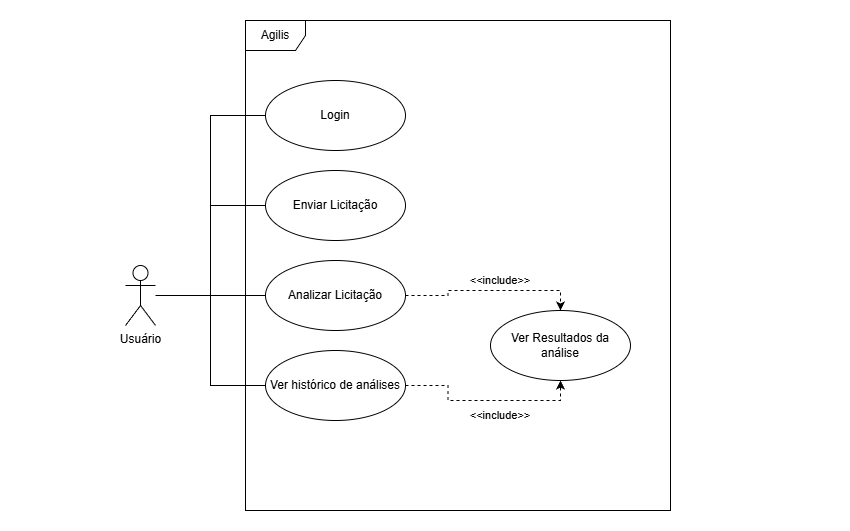
\includegraphics[width=0.8\textwidth]{Textuais/Figuras/agilis-usecase.png}
    \caption{Diagrama de casos de uso do sistema \textit{Agilis Licitações}.}
    \label{fig:caso_uso_agilis}
    \fonte{\me{2025}} % Elaborada pelo autor
\end{figure}


\subsection{Aderência aos Requisitos da Linha de Projeto}

O projeto \textit{Agilis Licitações} atende aos critérios obrigatórios da categoria \textbf{Projetos com Inteligência Artificial (IA)} pelos seguintes aspectos:

\begin{itemize}
    \item Emprega múltiplos algoritmos de inteligência artificial para processamento de texto, alinhados à evolução recente de modelos de linguagem \cite{devlin_bert_2019, chalkidis_legalbert_2020};
    \item Aplica técnicas de \textit{machine learning} e NLP na análise de documentos jurídicos \cite{hendrycks_lexnlp_2020};
    \item Utiliza arquitetura híbrida com Node.js e Python FastAPI, integrando backend com módulos inteligentes \cite{nodejs_docs_2024, fastapi_docs_2024};
    \item Define métricas de acurácia, desempenho e estabilidade para avaliação do modelo de IA.
\end{itemize}


\subsection{Ambiente de Treinamento e Conjunto de Dados}

O treinamento dos modelos de inteligência artificial do \textit{Agilis Licitações} será realizado majoritariamente em ambiente local, utilizando a estação de trabalho do autor para experimentos iniciais, ajustes de hiperparâmetros e testes de menor porte. Para treinamentos mais pesados, que demandem maior capacidade computacional, será utilizado o \textit{Google Colab Pro}, aproveitando recursos de GPU em nuvem. Em casos específicos que exijam processamento intensivo ou execução em larga escala, está previsto o uso de infraestrutura em nuvem na \textit{Amazon Web Services (AWS)}, de forma pontual, quando necessário.

O conjunto de treino será composto por editais públicos de licitação e por uma base de dados anotada manualmente, contendo as informações essenciais extraídas desses documentos (prazos, documentos exigidos, itens licitados, critérios de participação, entre outros). Essas anotações serão fornecidas pela empresa \textit{Amoveri Farma S.a.}, com base em licitações passadas que a empresa já analisou. O objetivo é alcançar um conjunto com aproximadamente \textbf{1.000 editais} anotados, estabelecendo como mínimo viável uma base de \textbf{300 editais} para os primeiros experimentos.

Todos os editais utilizados são documentos públicos, conforme estabelecido pela Lei nº 14.133/2021, que determina a obrigatoriedade de publicidade e divulgação eletrônica dos editais de licitação em plataformas oficiais como o PNCP \cite{brasil_lei_14133_2021}. As informações anotadas referem-se apenas a requisitos e regras de participação em licitações já encerradas, não contendo dados pessoais sensíveis. Dessa forma, o conjunto de treino não envolve tratamento de informações sigilosas ou protegidas pela LGPD, mantendo o foco apenas em dados jurídicos e administrativos de domínio público.

\section{Pipeline de Algoritmos de IA}

O núcleo inteligente do \textit{Agilis Licitações} é estruturado como uma \textit{pipeline} sequencial de algoritmos, no qual cada etapa refina o resultado da anterior, desde a leitura do edital em PDF até a geração de uma saída estruturada em formato JSON. Esse encadeamento permite combinar regras determinísticas, técnicas clássicas de processamento de texto e modelos de linguagem modernos, explorando o melhor de cada abordagem em termos de precisão, desempenho e robustez.

\begin{enumerate}
    \item \textbf{Ingestão e normalização do texto}\\
    Inicialmente, os arquivos de edital enviados pelo usuário (pode ser apenas um ou múltiplos PDFs) são unificados em um único documento lógico, quando necessário. Em seguida, bibliotecas especializadas como \textit{pdfplumber} e \textit{PyMuPDF} são utilizadas para extrair o texto bruto dos PDFs, de acordo com as práticas clássicas de parsing de documentos PDF \cite{hassan2016pdfparsing}, descartando elementos gráficos e mantendo apenas o conteúdo textual relevante. Sobre esse texto é aplicado um conjunto de regras de normalização, incluindo a padronização de quebras de linha, remoção de espaçamentos irregulares e recomposição de linhas que foram quebradas no meio de frases, resultando em um texto contínuo e adequado para processamento posterior.

    \item \textbf{Segmentação inteligente em seções}\\
    Para contornar limitações de \textit{context window} de modelos de linguagem \cite{beltagy2020longformer} e evitar o processamento de documentos extremamente extensos como um único bloco, o sistema realiza a segmentação do edital em seções coerentes \cite{utiyama2001segmentation}. Essa etapa combina heurísticas baseadas em expressões regulares e padrões típicos de editais (títulos em caixa alta, numeração hierárquica, expressões como ``DO OBJETO'', ``DAS CONDIÇÕES DE PARTICIPAÇÃO'' etc.) com um classificador leve baseado em modelos do tipo \textit{BERT}/\textit{LegalBERT} \cite{devlin_bert_2019, chalkidis_legalbert_2020}. As heurísticas identificam candidatos a início de seção e o classificador supervisionado decide, para cada candidato, se há de fato uma fronteira de seção, reduzindo o risco de cortar informações importantes ou fragmentar cláusulas relacionadas.

    \item \textbf{Localização de trechos candidatos}\\
    Com o edital segmentado em seções menores, o sistema precisa localizar onde, dentro do texto, estão as informações de interesse (prazos, documentos exigidos, itens licitados, critérios de participação etc.). Essa etapa começa com um módulo de \textbf{dicionário de termos}, que busca palavras-chave e expressões jurídicas ou técnicas pré-cadastradas, marcando seções potencialmente relevantes para cada tipo de informação. Em seguida, um módulo de \textbf{busca semântica com \textit{embeddings}} transforma parágrafos em vetores e compara esses vetores com consultas semânticas pré-definidas (por exemplo, ``prazo para apresentação das propostas'', ``documentos necessários para habilitação''). Um algoritmo de ranqueamento combina os resultados do dicionário e da busca semântica, produzindo um conjunto reduzido de trechos candidatos para cada categoria de informação.

    \item \textbf{Extração fina das informações}\\
    A etapa seguinte é responsável por extrair, de cada trecho candidato, os valores específicos que serão apresentados ao usuário (datas, listas de documentos, descrições de itens, percentuais, valores, entre outros). Para isso, o sistema utiliza um modelo de extração baseado em transformadores com \textit{fine tuning} supervisionado, seguindo a arquitetura e práticas descritas por \cite{wolf2020transformers}, treinado sobre o conjunto de editais anotados manualmente pela empresa \textit{Amoveri Farma S.a.}. Esse modelo recebe como entrada o trecho candidato e o tipo de informação a ser extraída, retornando os \textit{spans} de texto mais prováveis que contenham a resposta. Em paralelo, um módulo complementar baseado em expressões regulares é empregado para identificar e normalizar padrões específicos, como datas, valores monetários, CNPJ e números de processo, garantindo consistência de formato e maior confiança nos dados estruturados.

    \item \textbf{Consolidação e organização dos resultados}\\
    Por fim, os resultados extraídos passam por uma etapa de consolidação, na qual são combinados scores de confiança do modelo de extração, sinais da busca semântica e presença de termos do dicionário, a fim de selecionar os melhores valores por campo e resolver possíveis ambiguidades. Em seguida, um módulo leve baseado em modelo de linguagem (\textit{LLM}) é utilizado apenas para organizar as informações em uma estrutura JSON padronizada e, opcionalmente, gerar resumos explicativos para apresentação no frontend. O uso desse LLM é inspirado no papel de modelos de linguagem de grande porte na formatação e organização textual, conforme demonstrado em \cite{brown2020language}. O LLM opera sobre os dados já extraídos, não como fonte primária de decisão, reduzindo o risco de alucinações e garantindo que o sistema permaneça fiel ao conteúdo original dos editais.
\end{enumerate}

Essa sequência de algoritmos forma um fluxo de processamento completo, onde cada módulo tem uma responsabilidade clara e contribui para refinar a interpretação dos editais.

\begin{figure}[!htbp]
    \centering
    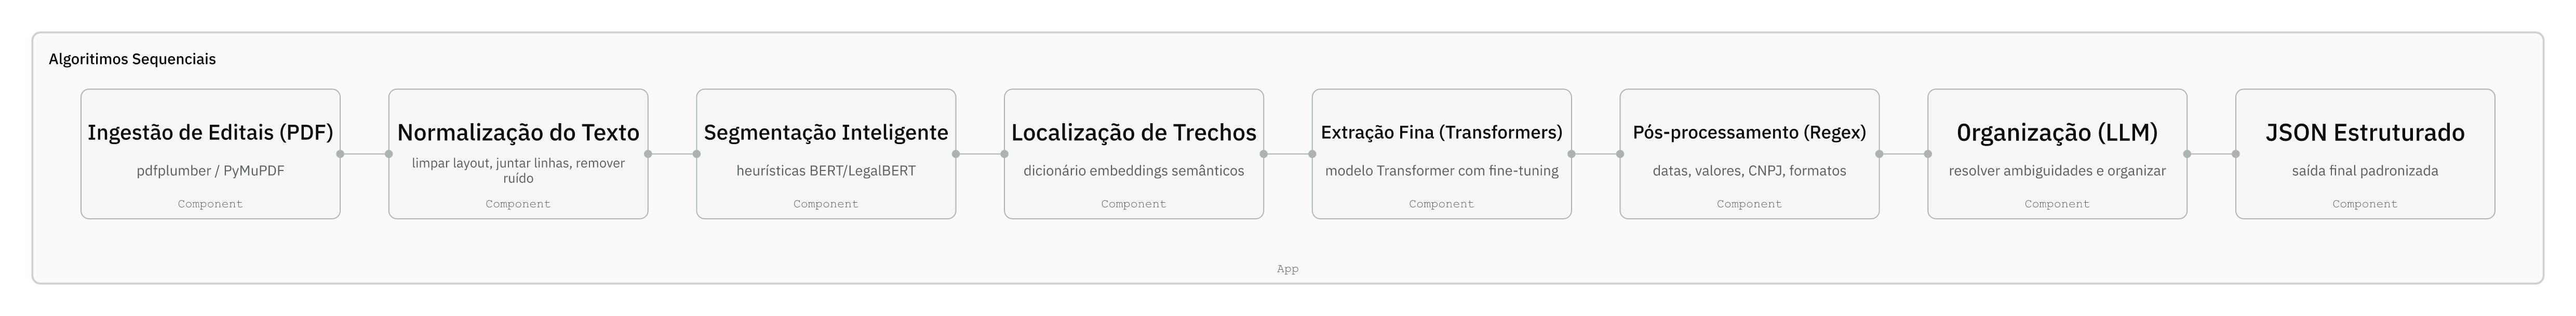
\includegraphics[width=0.95\textwidth]{Textuais/Figuras/Algoritimos-Sequenciais-Agilis-Att.png}
    \caption{Pipeline de algoritmos do sistema \textit{Agilis Licitações}.}
    \label{fig:pipeline_agilis}
    \fonte{\me{2025}}
\end{figure}


% -------------------------------------------------------------
\section{Considerações de Design}

\subsection{Visão Inicial da Arquitetura}

O sistema segue uma arquitetura modular em camadas, composta pelos seguintes componentes principais, em conformidade com princípios de arquitetura de software orientada a responsabilidade e separação de camadas \cite{bass_software_architecture_2012}:

\begin{itemize}
    \item \textbf{Interface Visual (Frontend — React):} permite o upload de arquivos, o login de usuários e a visualização dos resultados das análises \cite{react_docs_2024};
    
    \item \textbf{Servidor Principal (Backend — Express.js):} gerencia autenticação, requisições, armazenamento de dados e a comunicação com o módulo de IA \cite{nodejs_docs_2024};
    
    \item \textbf{Módulo de IA (FastAPI — Python):} executa os algoritmos de leitura, extração textual, análise, lógica, expressões regulares, NLP e aprendizado de máquina \cite{fastapi_docs_2024};
    
    \item \textbf{Banco de Dados (PostgreSQL):} armazena usuários, logs, resultados de análises e hashes de verificação para evitar reprocessamentos \cite{postgresql_docs_2024}.
\end{itemize}


\subsection{Padrões de Arquitetura}

O sistema adota uma \textbf{Arquitetura em Camadas}, separando responsabilidades de forma clara entre os módulos. Esse padrão facilita a manutenção, a escalabilidade e a organização do código, além de permitir a evolução independente de cada componente \cite{bass_software_architecture_2012}.

As camadas utilizadas são:

\begin{itemize}
    \item \textbf{Camada de Apresentação (Frontend — React):} responsável pela interação com o usuário, envio de arquivos e exibição dos resultados;
    
    \item \textbf{Camada de Aplicação (Backend — Express.js):} coordena o fluxo de requisições, autenticação, regras de negócio e comunicação com o módulo de IA;
    
    \item \textbf{Camada de Serviço de IA (FastAPI — Python):} executa os algoritmos de análise textual, NLP, lógica e aprendizado de máquina;
    
    \item \textbf{Camada de Dados (PostgreSQL):} armazena usuários, resultados de análises, logs e informações persistentes do sistema.
\end{itemize}


\subsection{Modelo Entidade Relacionamento}

A Figura~\ref{fig:mer_agilis} apresenta o Modelo Entidade-Relacionamento (MER) do sistema \textit{Agilis Licitações}, descrevendo as entidades principais e suas relações. O modelo inclui as entidades \textbf{Usuário}, \textbf{Edital} e \textbf{Análise}, permitindo registrar quem realizou cada análise, qual edital foi processado e os resultados obtidos.

\begin{figure}[!htbp]
    \centering
    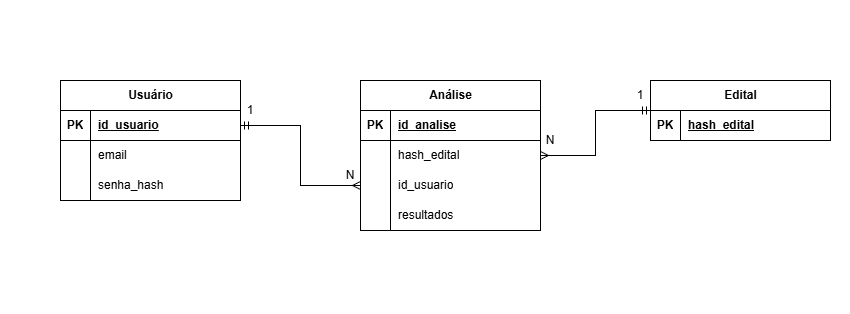
\includegraphics[width=0.95\textwidth]{Textuais/Figuras/modeloentidaderelacionamento.png}
    \caption{Modelo Entidade-Relacionamento do sistema \textit{Agilis Licitações}.}
    \label{fig:mer_agilis}
    \fonte{\me{2025}} % Elaborada pelo autor
\end{figure}


\subsection{Diagramas}

Os diagramas desta seção representam a arquitetura do sistema utilizando o \textit{C4 Model} \cite{brown_c4_model_2018} nos níveis de Contexto, Containers e Componentes, além do Modelo Entidade-Relacionamento apresentado anteriormente. Os diagramas foram produzidos com o objetivo de facilitar o entendimento estrutural e operacional do \textit{Agilis Licitações}.

\paragraph{C4 — Nível 1 (Contexto)}
A Figura~\ref{fig:c4_contexto} apresenta a visão de contexto do sistema, destacando a interação entre o usuário e o \textit{Agilis Licitações}.

\begin{figure}[!htbp]
    \centering
    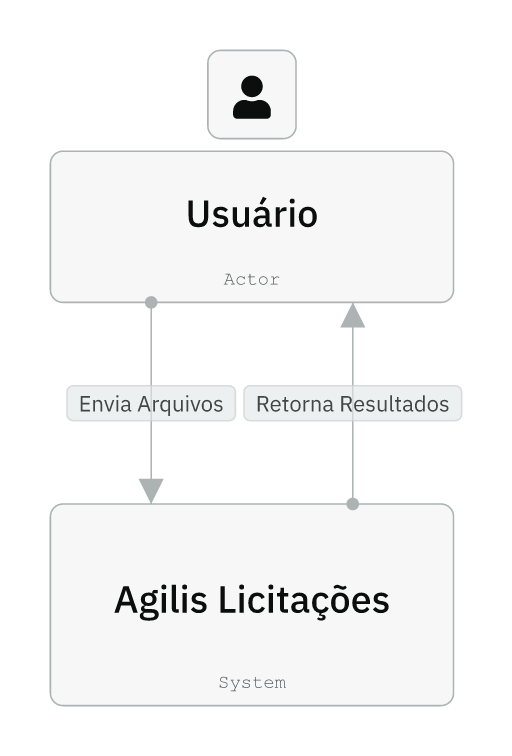
\includegraphics[width=0.75\textwidth]{Textuais/Figuras/c4model-context.png}
    \caption{C4 Model — Nível 1 (Contexto) do sistema \textit{Agilis Licitações}.}
    \label{fig:c4_contexto}
    \fonte{\me{2025}}
\end{figure}

\paragraph{C4 — Nível 2 (Containers)}
A Figura~\ref{fig:c4_containers} apresenta os containers do sistema, incluindo frontend, backend, módulo de IA e banco de dados, com suas responsabilidades e fluxos de comunicação.

\begin{figure}[!htbp]
    \centering
    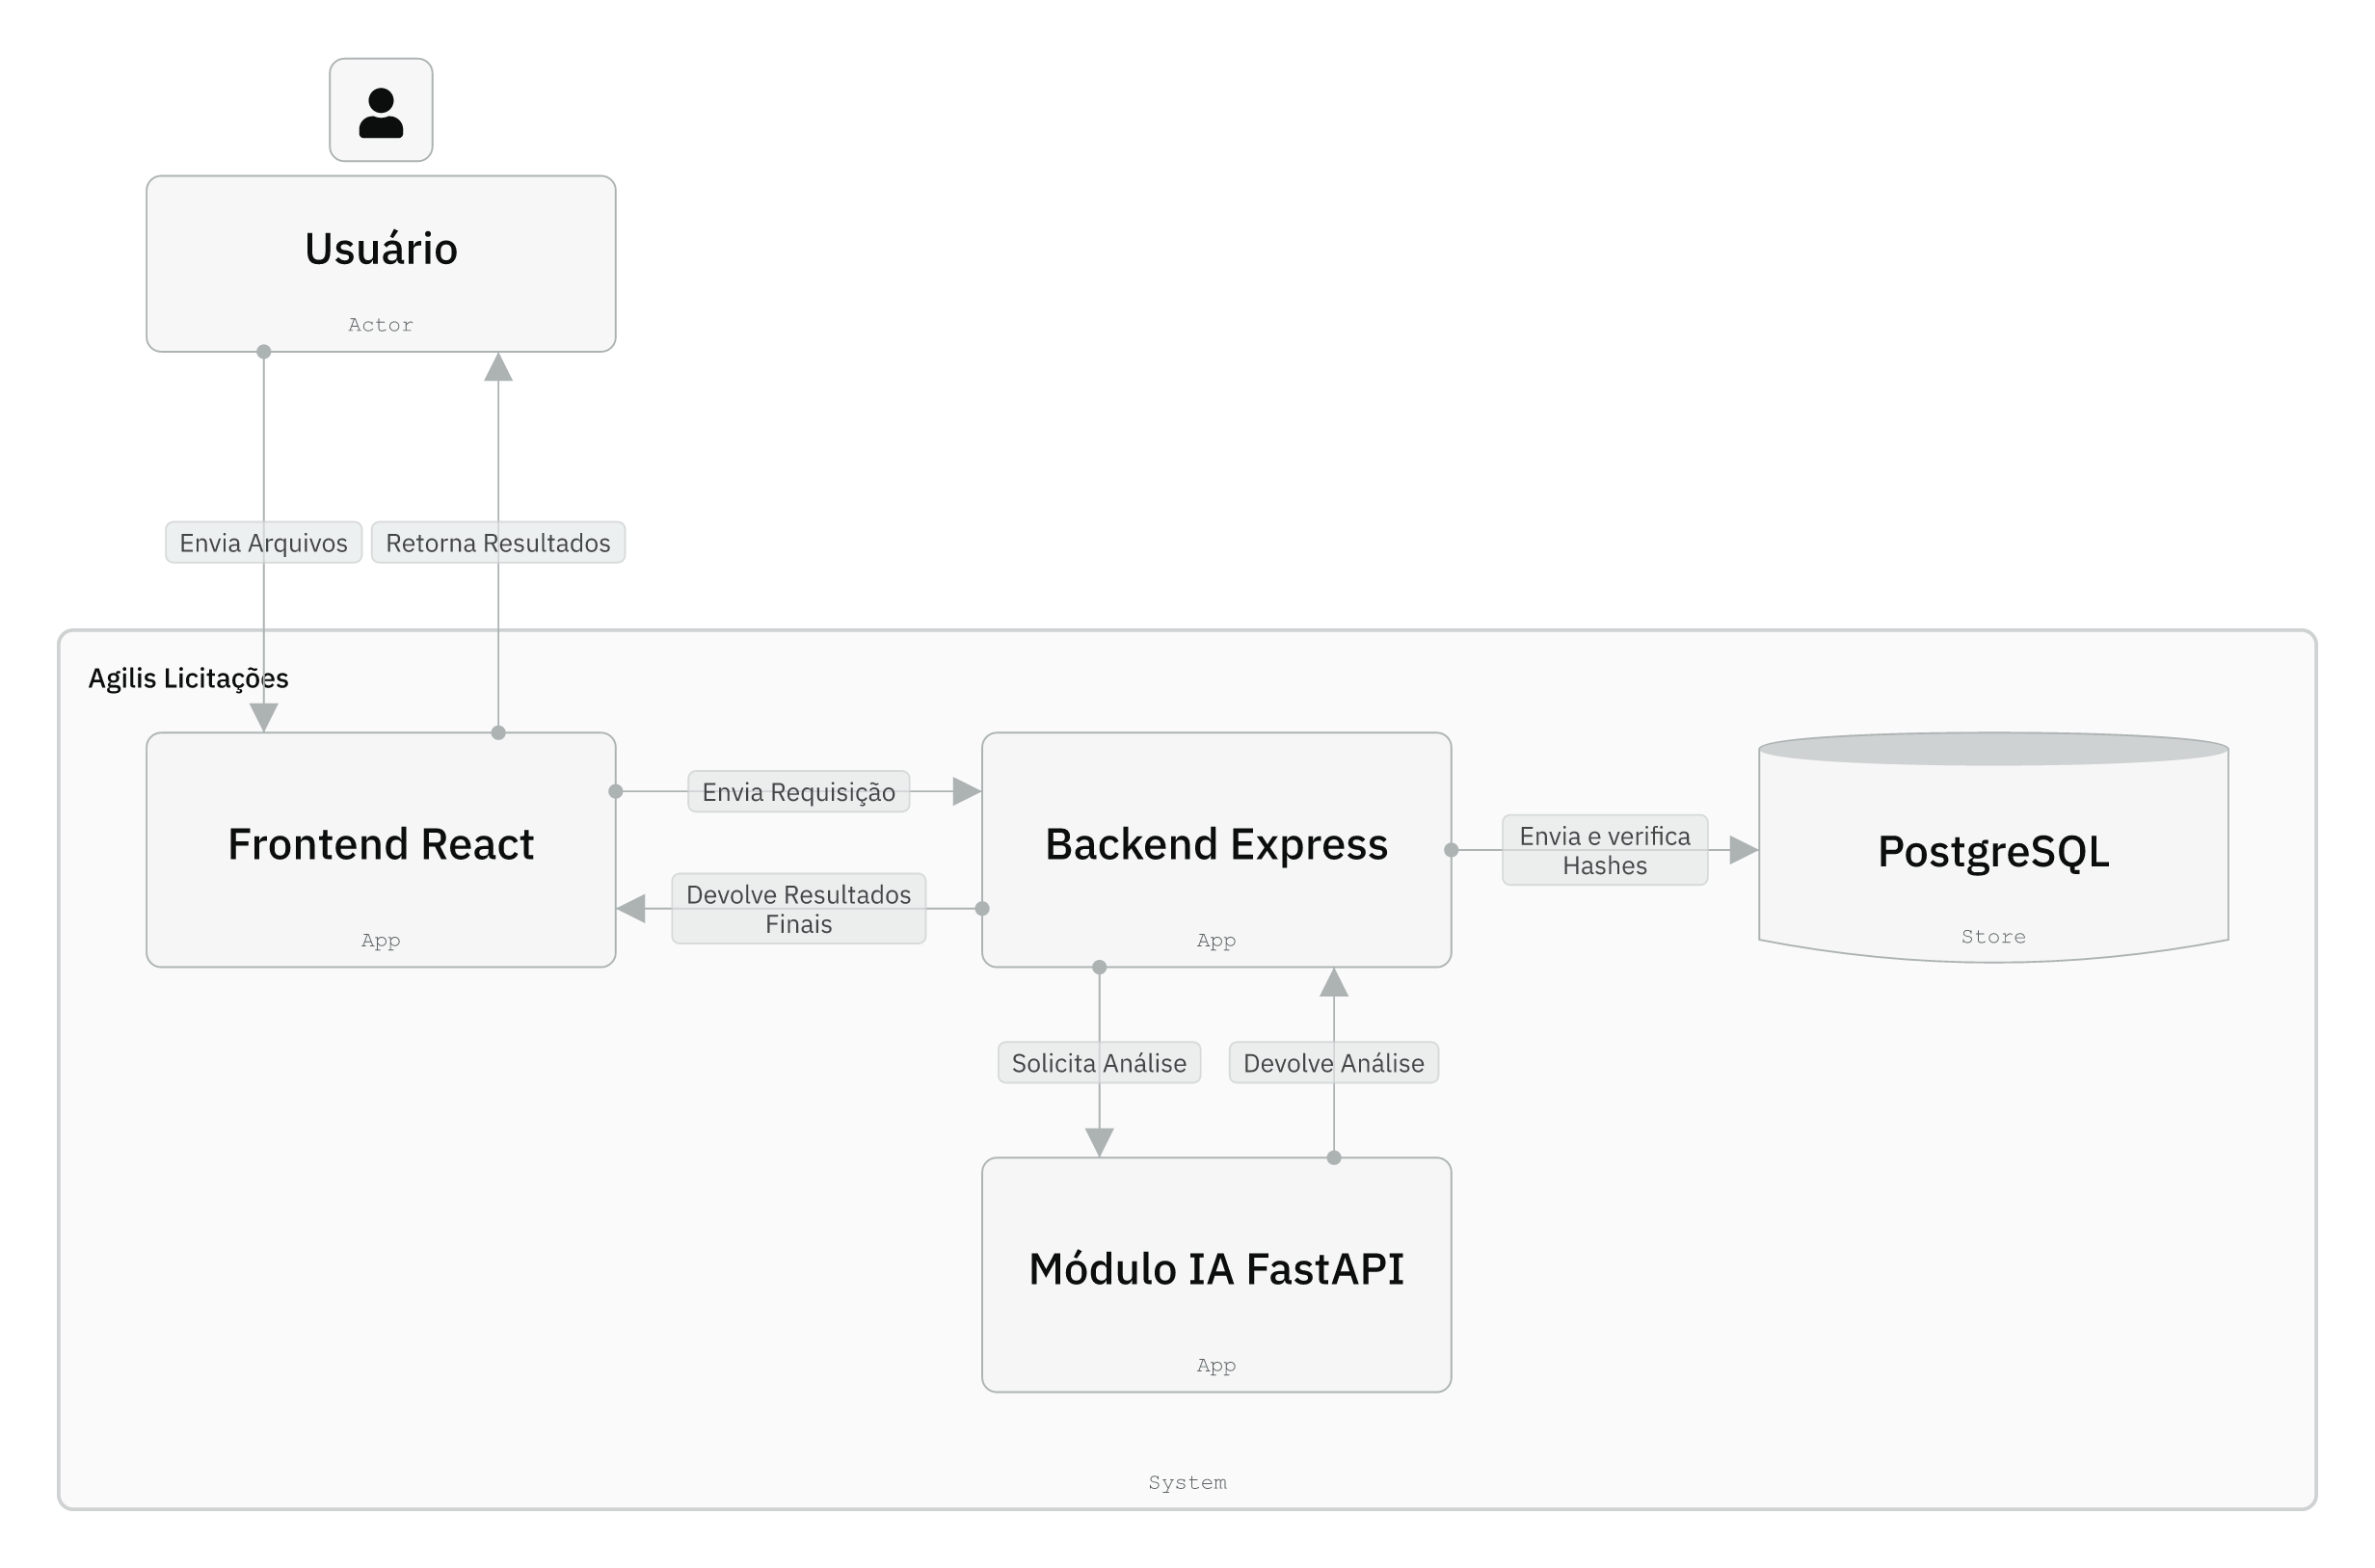
\includegraphics[width=0.95\textwidth]{Textuais/Figuras/c4model-app.png}
    \caption{C4 Model — Nível 2 (Containers) do sistema \textit{Agilis Licitações}.}
    \label{fig:c4_containers}
    \fonte{\me{2025}}
\end{figure}

\paragraph{C4 — Nível 3 (Componentes do Backend)}
A Figura~\ref{fig:c4_componentes} detalha os principais componentes internos do \textit{Backend Express}, incluindo controladores, serviços auxiliares e comunicação com o módulo de IA e o banco de dados.

\begin{figure}[!htbp]
    \centering
    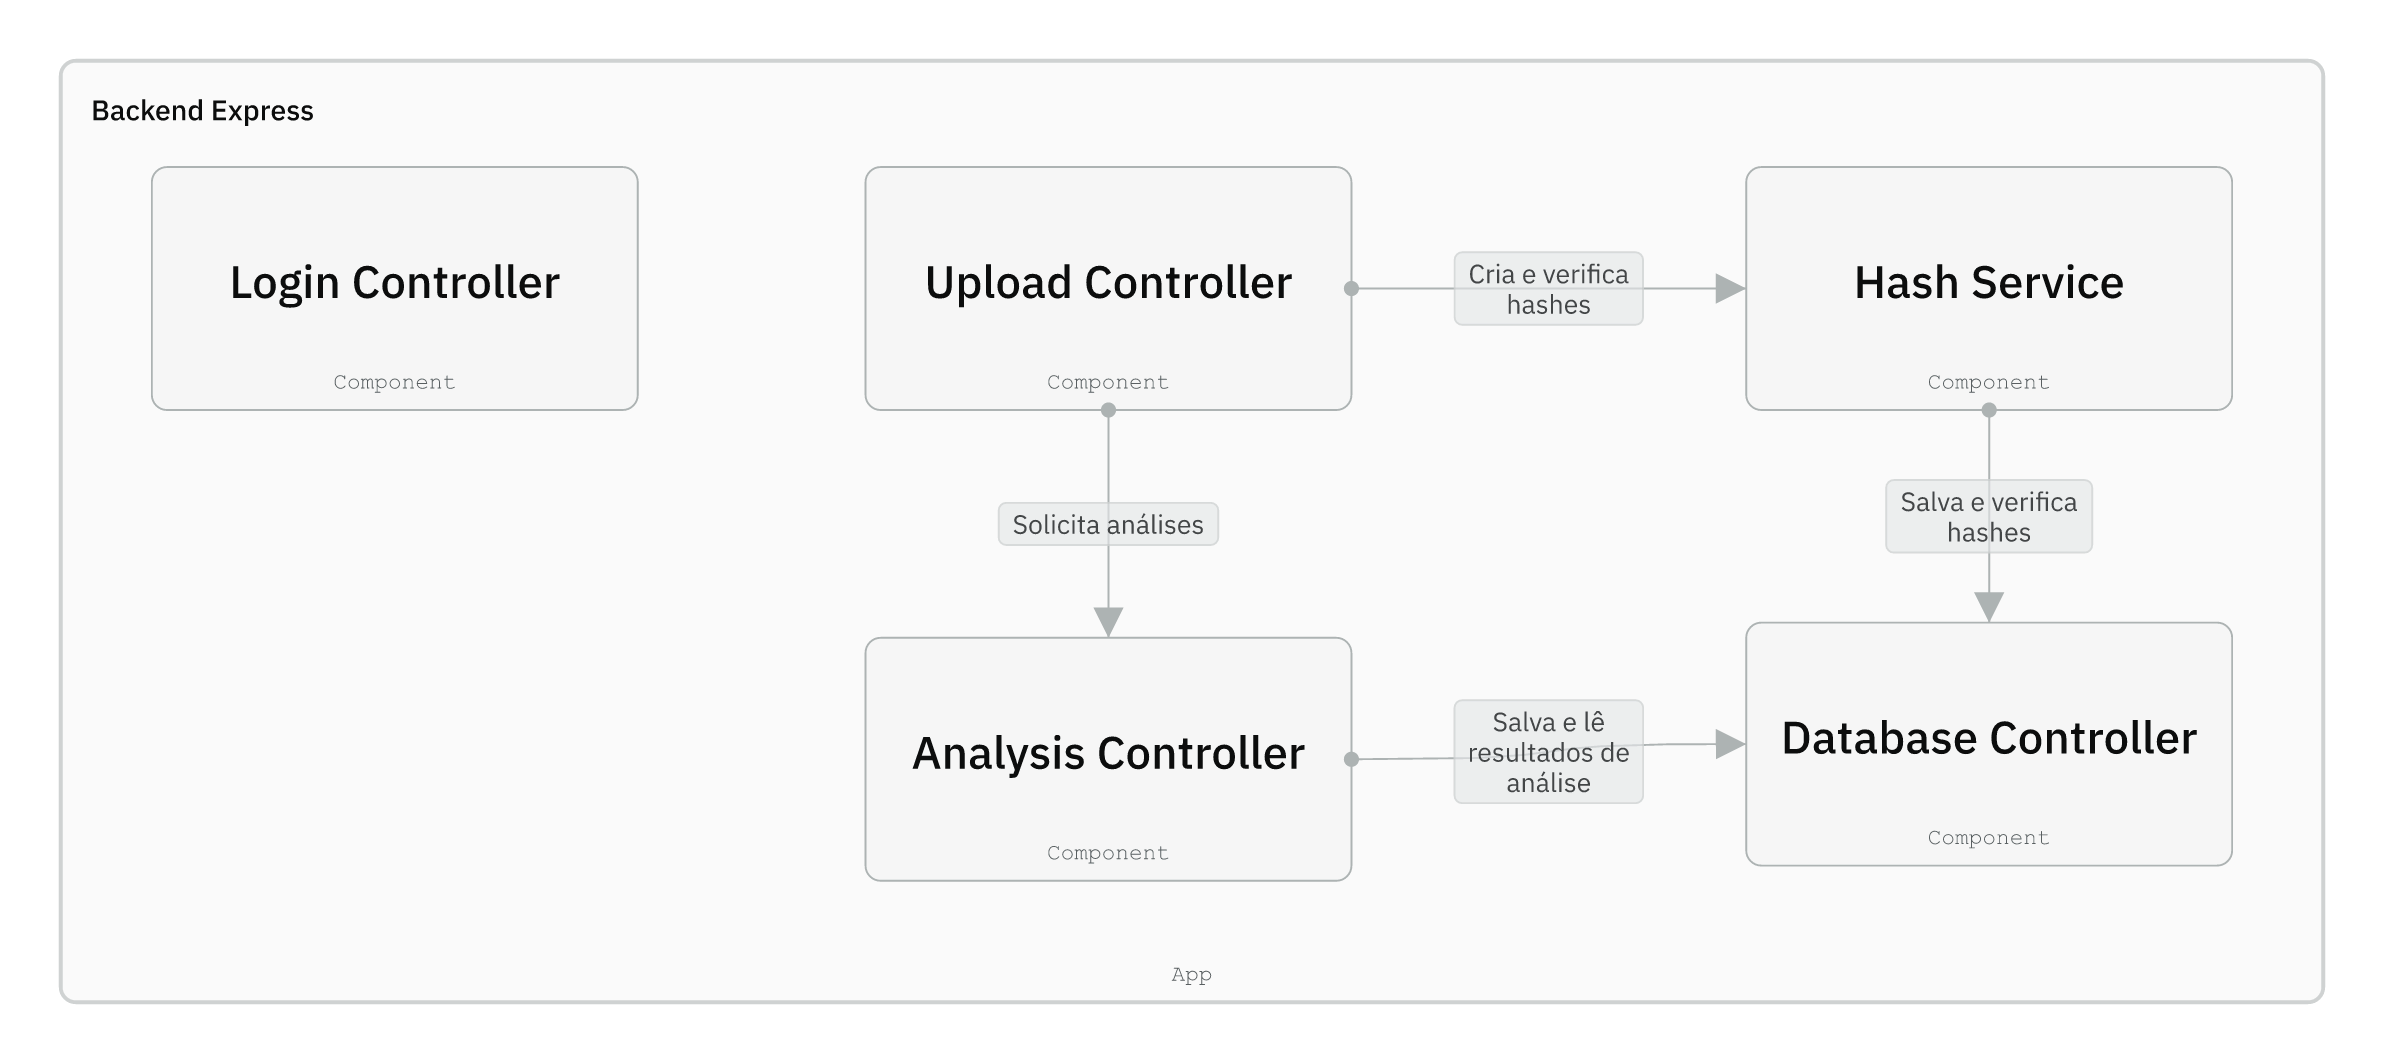
\includegraphics[width=0.95\textwidth]{Textuais/Figuras/c4model-component.png}
    \caption{C4 Model — Nível 3 (Componentes do Backend Express).}
    \label{fig:c4_componentes}
    \fonte{\me{2025}}
\end{figure}



\subsection{Mockups das Telas Principais}

As principais telas do sistema foram prototipadas para representar o fluxo de uso previsto no \textit{Agilis Licitações}. Os mockups a seguir demonstram as interfaces de acesso, análise e visualização dos resultados.

\paragraph{Tela de Login}
A Figura~\ref{fig:mockup_login} apresenta a tela de login do sistema, onde o usuário informa suas credenciais de acesso para entrar na plataforma e iniciar as análises.

\begin{figure}[!htbp]
    \centering
    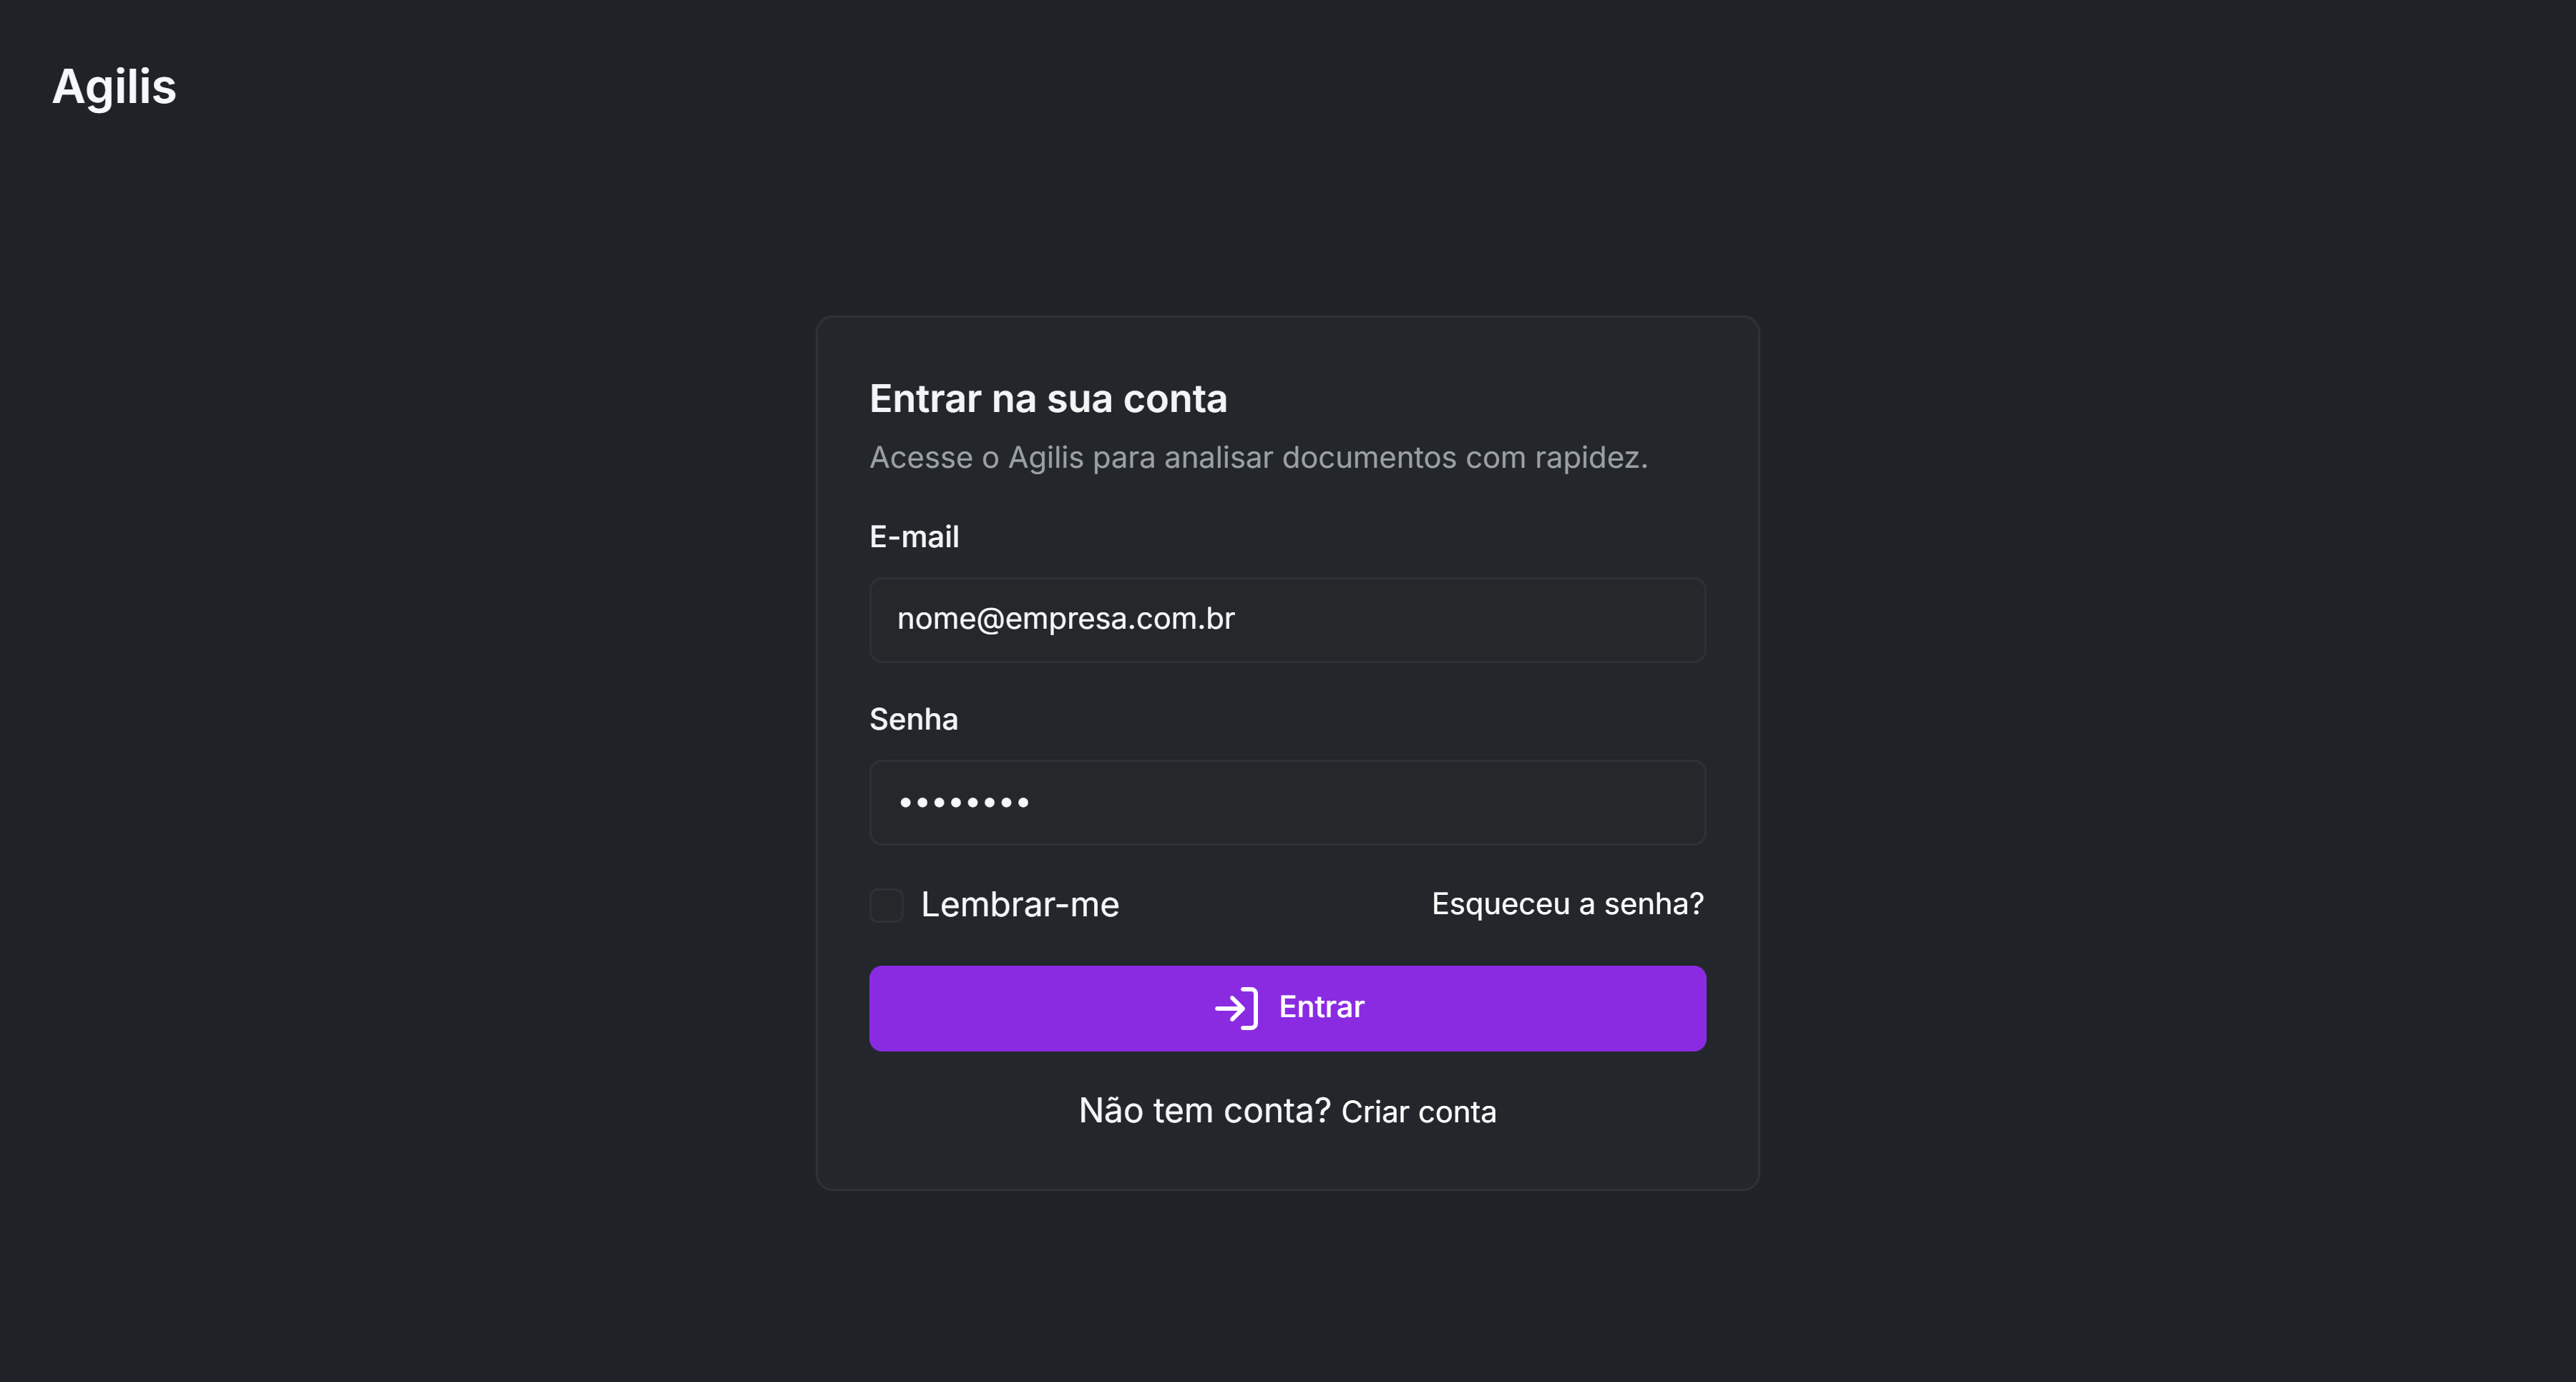
\includegraphics[width=0.95\textwidth]{Textuais/Figuras/LoginScreen.png}
    \caption{Mockup da tela de login do sistema \textit{Agilis Licitações}.}
    \label{fig:mockup_login}
    \fonte{\me{2025}}
\end{figure}

\paragraph{Tela de Análise em Execução}
A Figura~\ref{fig:mockup_analisando} mostra o estado de processamento do edital, indicando ao usuário que o sistema está executando os algoritmos de análise.

\begin{figure}[!htbp]
    \centering
    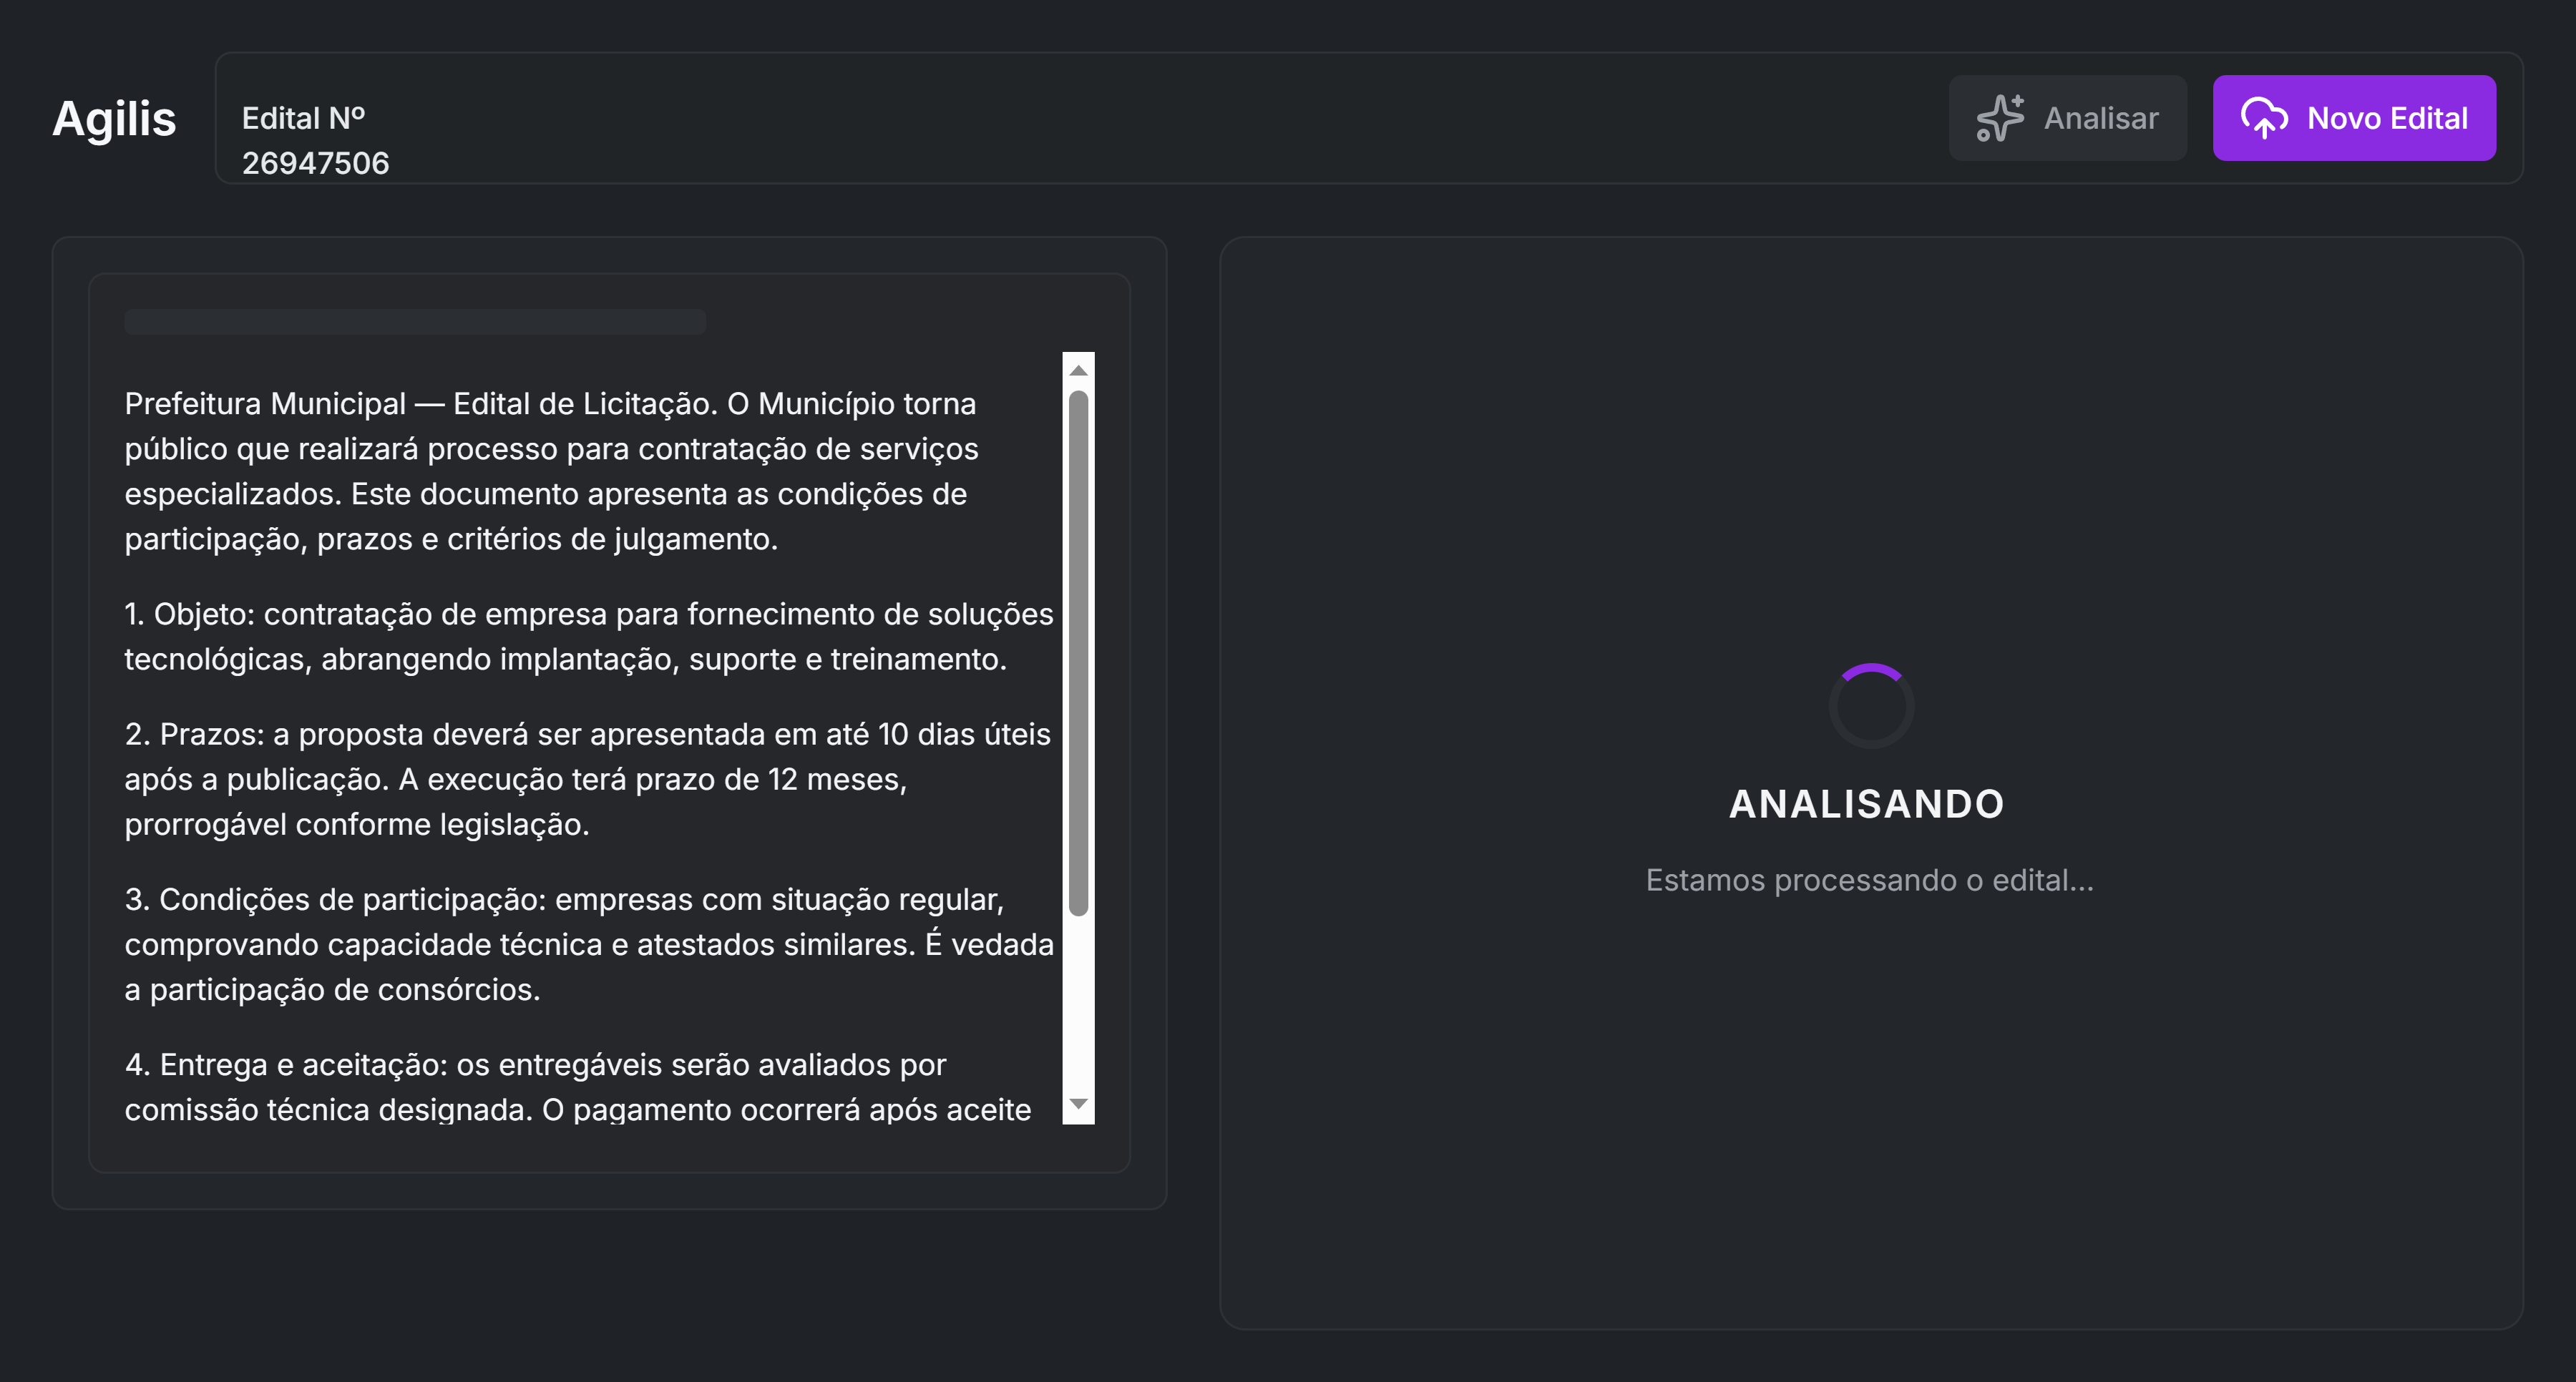
\includegraphics[width=0.95\textwidth]{Textuais/Figuras/AnalyzingState.png}
    \caption{Mockup da tela de análise em execução.}
    \label{fig:mockup_analisando}
    \fonte{\me{2025}}
\end{figure}

\paragraph{Tela de Resultados}
A Figura~\ref{fig:mockup_resultados} apresenta a tela onde o usuário visualiza o edital enviado e os resultados extraídos automaticamente, incluindo critérios de habilitação, prazos, riscos e recomendações.

\begin{figure}[!htbp]
    \centering
    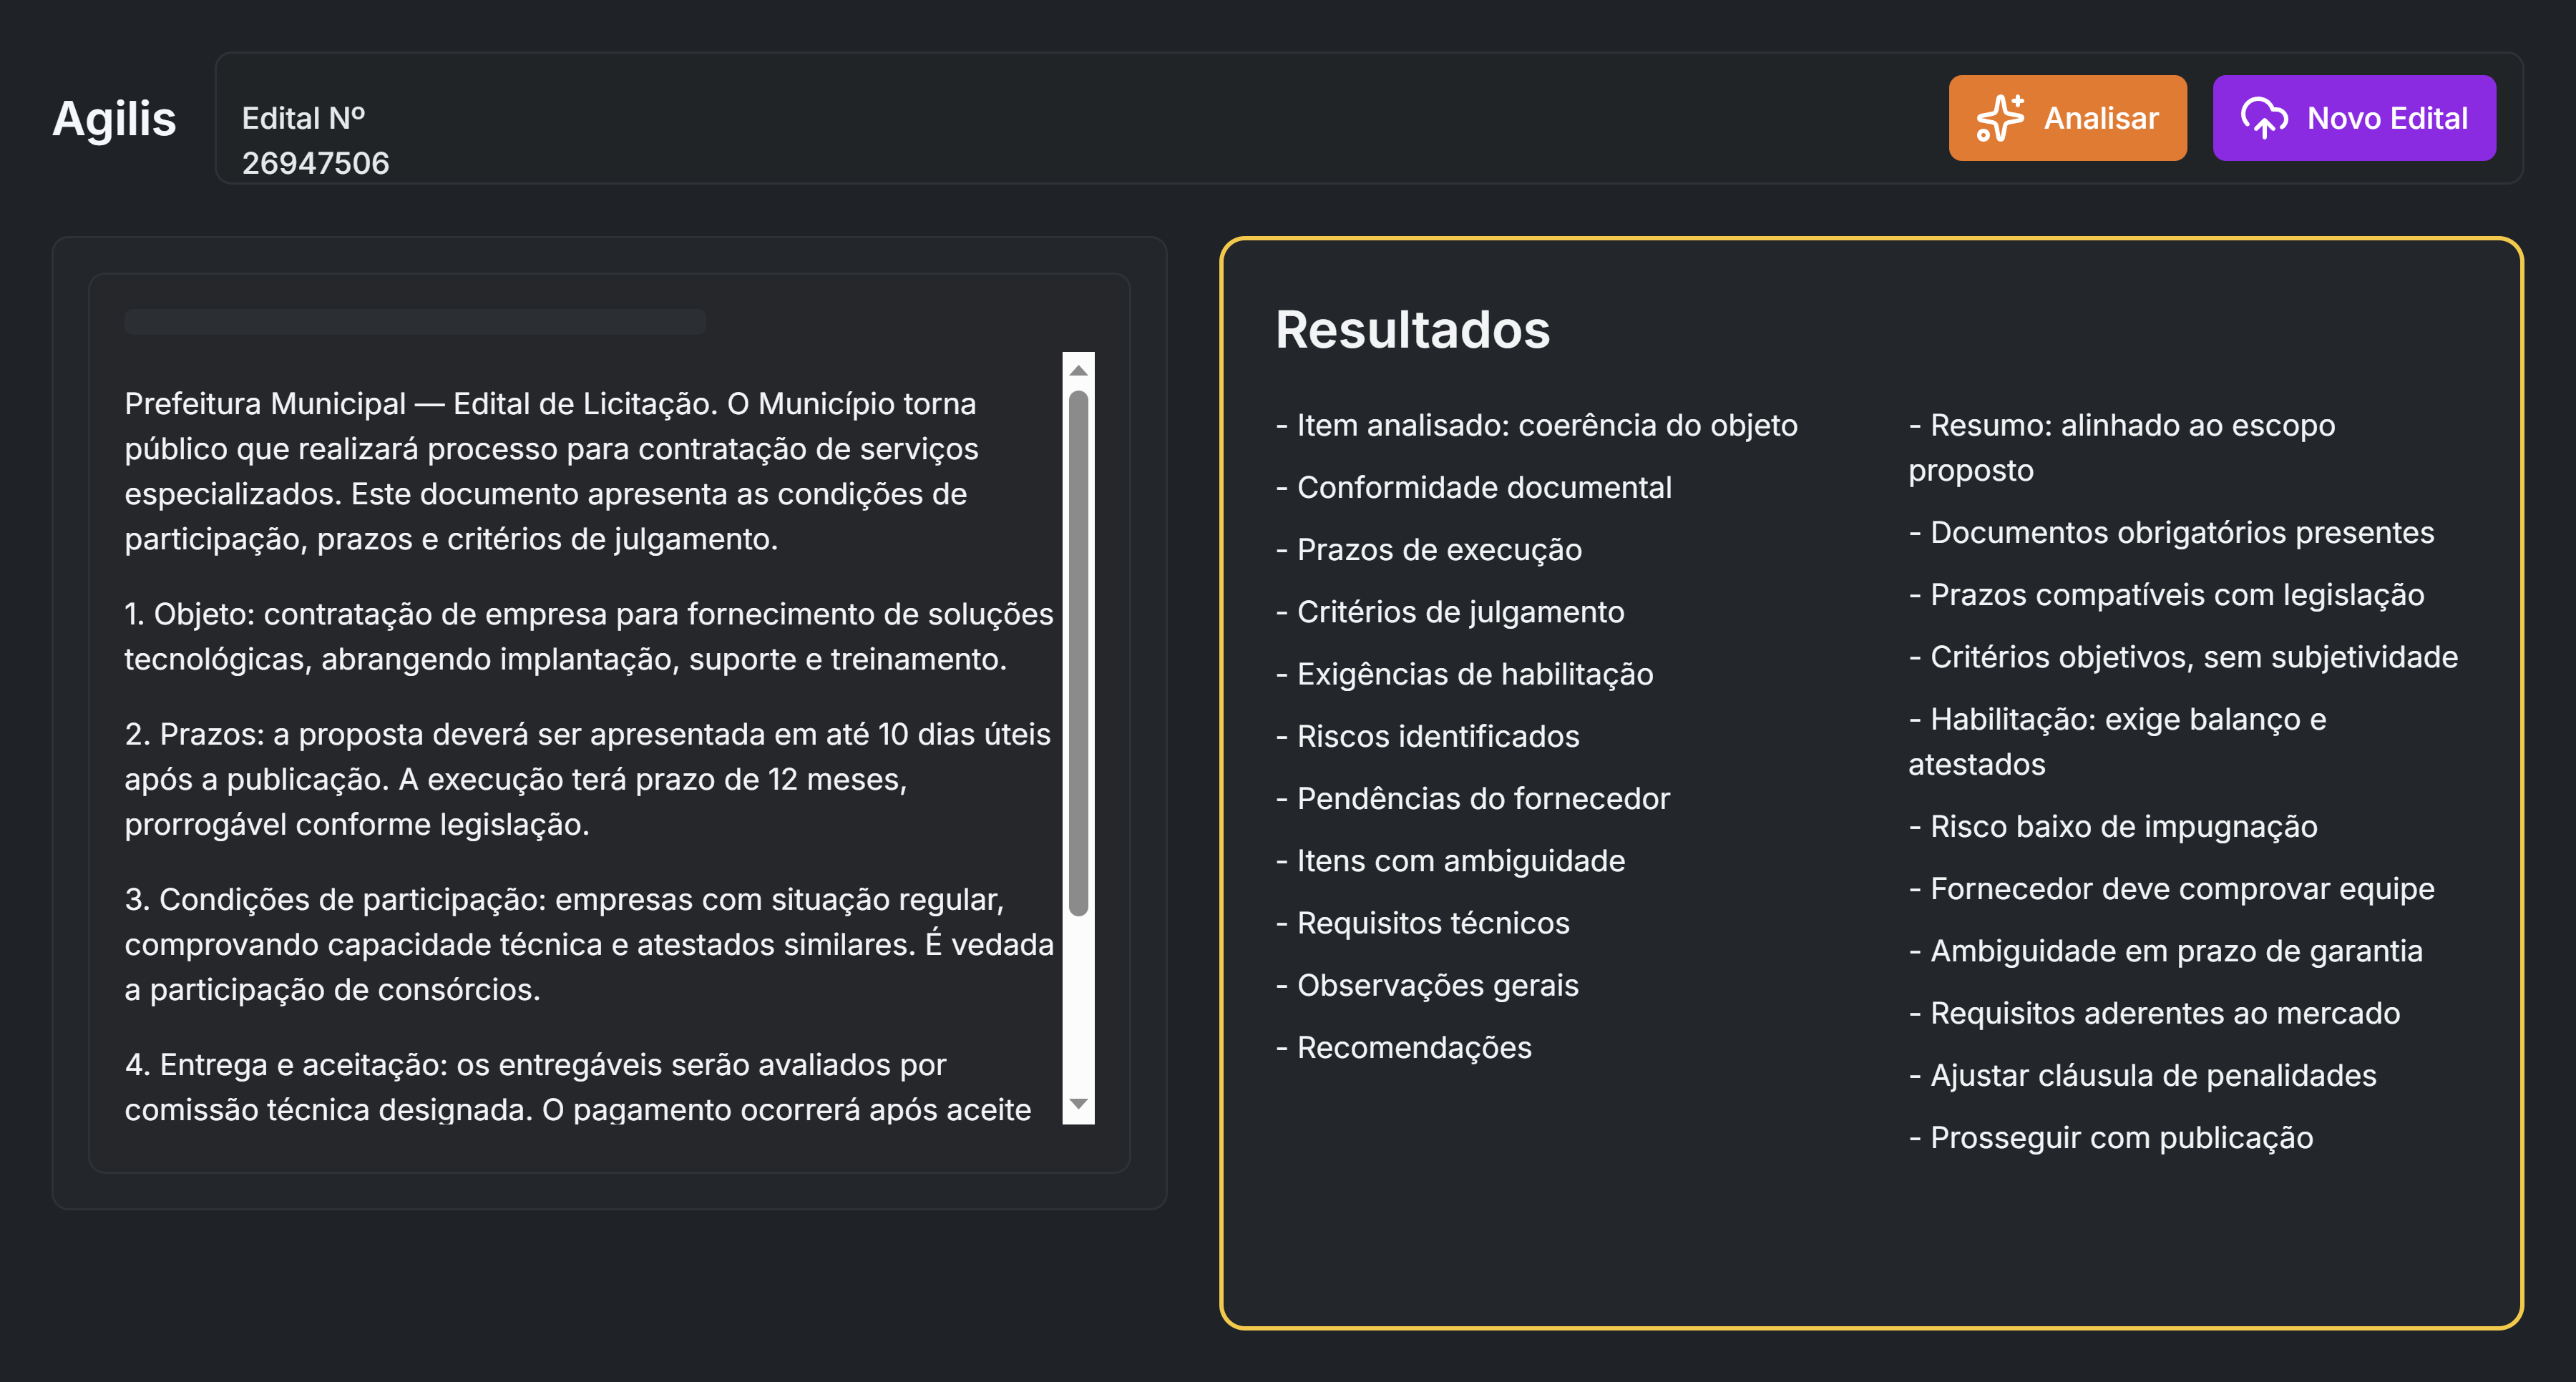
\includegraphics[width=0.95\textwidth]{Textuais/Figuras/AnaliseEdital.png}
    \caption{Mockup da tela de visualização dos resultados da análise.}
    \label{fig:mockup_resultados}
    \fonte{\me{2025}}
\end{figure}


\subsection{Decisões e Alternativas Consideradas}

A arquitetura híbrida adotada combina Node.js no backend principal e Python (FastAPI) no módulo de IA. Essa escolha foi motivada pela eficiência do Node.js em operações assíncronas, gerenciamento de requisições e integração com o frontend \cite{nodejs_docs_2024}, enquanto o Python oferece robustez e maturidade em bibliotecas de processamento de linguagem natural, aprendizado de máquina e análise textual \cite{python_docs_2024, pandas_docs_2024}. No frontend, o uso de React e bibliotecas de componentes como \textit{shadcn/ui} favorece produtividade e consistência visual \cite{react_docs_2024, shadcn_docs_2024}.

Como alternativa, foi avaliada a construção de todo o sistema em uma única linguagem, utilizando frameworks Python como Django ou Flask. No entanto, essa abordagem foi descartada devido à menor flexibilidade em cenários de alto volume de requisições assíncronas e à integração menos fluida com o ecossistema moderno de desenvolvimento web. A separação dos módulos permitiu maior desempenho, modularidade e independência tecnológica entre as camadas \cite{bass_software_architecture_2012}.


\subsection{Critérios de Escalabilidade, Resiliência e Segurança}

Os critérios adotados visam garantir que o sistema possa crescer, lidar com falhas e manter a segurança dos dados dos usuários e dos processos de análise.

\begin{itemize}
    \item \textbf{Escalabilidade:} o sistema é hospedado em um servidor centralizado, permitindo acesso remoto simples e possibilidade de expansão futura por meio de réplicas do backend ou do módulo de IA, caso haja aumento de demanda;
    
    \item \textbf{Resiliência:} o backend Express.js mantém registros de execução e logs de erro para identificação de falhas, possibilitando correções rápidas e facilitando a monitoração contínua do funcionamento do sistema;
    
    \item \textbf{Segurança:} as credenciais são armazenadas com hashing criptográfico, a autenticação é realizada via JWT, e entradas do usuário passam por validação, em conformidade com a Lei Geral de Proteção de Dados (LGPD) \cite{brasil_lei_13709_2018} e com a especificação formal de tokens JWT \cite{jwt_rfc7519_2015}.
\end{itemize}


% -------------------------------------------------------------
\section{Ferramentas Tecnológicas}

\subsection{Linguagens de Programação}

As linguagens utilizadas no projeto foram escolhidas pela adequação às suas funções específicas dentro da arquitetura híbrida do sistema.

\begin{itemize}
    \item \textbf{JavaScript (Node.js e React):} escolhida pela versatilidade, ampla adoção no desenvolvimento web, facilidade de integração entre frontend e backend e suporte nativo a operações assíncronas \cite{nodejs_docs_2024, react_docs_2024};
    
    \item \textbf{Python (FastAPI):} utilizada no módulo de IA pela robustez em algoritmos complexos, disponibilidade de bibliotecas avançadas para NLP e aprendizado de máquina e excelente desempenho em tarefas de processamento textual \cite{python_docs_2024, fastapi_docs_2024}.
\end{itemize}


\subsection{Frameworks e Bibliotecas}

\begin{itemize}
    \item \textbf{Express.js:} utilizado no backend principal pela sua leveza, versatilidade e excelente desempenho em operações assíncronas, além da ampla compatibilidade com o ecossistema JavaScript \cite{nodejs_docs_2024};
    
    \item \textbf{FastAPI:} empregado no módulo de IA devido à sua alta performance em APIs Python, suporte nativo a validação de dados e integração simples com bibliotecas de processamento de linguagem natural \cite{fastapi_docs_2024};
    
    \item \textbf{Pandas:} utilizado para manipulação de dados e pré-processamento de textos, oferecendo alta compatibilidade com demais bibliotecas Python voltadas a análise e NLP \cite{pandas_docs_2024};
    
    \item \textbf{shadcn/ui:} adotado no frontend React para construção de interfaces visuais modernas, consistentes e com componentes reutilizáveis, acelerando o desenvolvimento das telas \cite{shadcn_docs_2024};
    
    \item \textbf{PostgreSQL:} utilizado como banco de dados relacional principal do sistema, devido à sua maturidade, estabilidade e licença permissiva \cite{postgresql_docs_2024};
    
    \item \textbf{Outras bibliotecas:} serão adicionadas conforme a evolução do projeto, especialmente ferramentas complementares para interface, validação, análise textual e integração entre módulos.
\end{itemize}


\subsection{Ferramentas de Desenvolvimento e Gestão}

As ferramentas adotadas no desenvolvimento do \textit{Agilis Licitações} foram escolhidas pela praticidade, integração com o fluxo de trabalho e suporte às tecnologias utilizadas no projeto.

\begin{itemize}
    \item \textbf{Visual Studio Code:} ambiente de desenvolvimento utilizado para edição de código, organização do projeto e integração com extensões voltadas a JavaScript e Python \cite{vscode_docs_2024};
    
    \item \textbf{GitHub:} plataforma de versionamento e colaboração utilizada para armazenar o código-fonte, controlar alterações e manter o histórico de desenvolvimento \cite{github_docs_2024};
    
    \item \textbf{Node.js e npm:} utilizados para gerenciamento de dependências do backend Express.js e do frontend React \cite{nodejs_docs_2024};
    
    \item \textbf{Python e pip:} empregados para gerenciar bibliotecas do módulo de IA desenvolvido em FastAPI \cite{python_docs_2024};
    
    \item \textbf{Insomnia:} ferramenta utilizada para teste, depuração e validação das APIs do backend e do módulo de IA durante o desenvolvimento \cite{insomnia_docs_2024}.
\end{itemize}


\subsection{Licenciamento}

As tecnologias utilizadas no desenvolvimento do \textit{Agilis Licitações} adotam licenças permissivas, permitindo modificação, distribuição e uso comercial sem grandes restrições.

\begin{itemize}
    \item \textbf{JavaScript, Node.js, React, Express.js e shadcn/ui:} licenciados sob \textbf{MIT}, permitindo uso livre e ampla flexibilidade no desenvolvimento;
    
    \item \textbf{FastAPI:} distribuído sob a licença \textbf{MIT}, favorecendo criação de APIs de forma aberta e permissiva;
    
    \item \textbf{Python:} licenciado sob a \textbf{Python Software Foundation License 2.0 (PSF)};
    
    \item \textbf{Pandas:} distribuído sob a licença \textbf{BSD-3-Clause};
    
    \item \textbf{PostgreSQL:} utiliza a \textbf{PostgreSQL License}, similar a licenças permissivas amplamente empregadas em software livre;
    
    \item \textbf{Insomnia:} licenciado sob \textbf{MIT}, permitindo uso livre como ferramenta de teste de APIs.
\end{itemize}


% -------------------------------------------------------------
\section{Considerações de Segurança}

\subsection{Riscos Identificados}

Os principais riscos associados ao funcionamento do sistema incluem:

\begin{itemize}
    \item Vazamento de credenciais de usuário;
    \item Injeção de código por entradas malformadas;
    \item Envio de arquivos potencialmente maliciosos ou não suportados;
    \item Falhas de autenticação ou uso indevido de tokens;
    \item Instabilidade causada por uploads excessivamente grandes ou acima do limite operacional.
\end{itemize}

\subsection{Medidas de Mitigação}

Para reduzir os riscos identificados, o sistema adota as seguintes medidas:

\begin{itemize}
    \item \textbf{Armazenamento seguro de credenciais}, utilizando hashing criptográfico;
    \item \textbf{Validação} dos dados de entrada em uploads e formulários;
    \item \textbf{Autenticação com tokens JWT}, garantindo controle de acesso seguro \cite{jwt_rfc7519_2015};
    \item \textbf{Restrição de tipos de arquivo}, permitindo apenas \textbf{PDF} e \textbf{TXT};
    \item \textbf{Limite de tamanho} de até \textbf{250 MB} por arquivo;
    \item \textbf{Limite de quantidade} de até \textbf{30 arquivos} por análise;
\end{itemize}

\subsection{Normas e Boas Práticas Seguidas}

O sistema segue diretrizes básicas de segurança recomendadas para aplicações web e serviços distribuídos, com foco no cumprimento da legislação vigente de proteção de dados:

\begin{itemize}
    \item \textbf{Diretrizes essenciais da LGPD}, aplicadas exclusivamente ao tratamento de dados de login e autenticação \cite{brasil_lei_13709_2018};
    \item \textbf{Separação entre módulos} (frontend, backend e módulo de IA), reduzindo exposição de serviços.
\end{itemize}

\subsection{Responsabilidade Ética}

Embora utilize inteligência artificial, o sistema opera exclusivamente sobre \textbf{documentos públicos}, não manipulando dados pessoais sensíveis. Dessa forma, mantém aderência a princípios éticos de privacidade, transparência e uso responsável de IA, em consonância com os fundamentos da LGPD \cite{brasil_lei_13709_2018}.
